algorithm:
\begin{enumerate}
	\item Calculate $ \hat{\vec{E}}_{0, \bot}^{ijn} $ via discrete Fourier transforms in time:
	\begin{equation}
	\omega^n = \frac{2 \pi}{N_t \delta t} \left( -\frac{N_t}{2} + n \right),
	\end{equation}
	\begin{equation}
	\hat{\vec{E}}_{0, \bot}^{ijn} = \frac{\delta t}{2 \pi} \sum_{l=1}^{N_t} \vec{E}_{0, \bot}^{ijl} \e^{\i \omega^n t^l}, \quad n \in \left\lbrace 1, \dots, N_t \right\rbrace.
	\end{equation}
	\item Calculate $ \bar{\vec{E}}_{0, \bot}^{ijn} $ via two-dimensional discrete Fourier transforms in transverse space:
	\begin{equation}
	k_x^i = \frac{2 \pi}{N_x \delta x} \left( - \frac{N_x}{2} + i\right), \quad k_y^j = \frac{2 \pi}{N_y \delta y} \left( - \frac{N_y}{2} + j\right),
	\end{equation}
	\begin{equation}
	\bar{\vec{E}}_{0, \bot}^{ijn} = \frac{\delta x \delta y}{(2 \pi)^2} \sum_{l, m = 1}^{N_x, N_y} \hat{\vec{E}}_{0, \bot}^{lmn} \e^{- \i \: \left(k_x^i x^l + k_y^j y^m \right)}, \quad i, j \in \left\lbrace 1, \dots, N_{x, y} \right\rbrace.
	\end{equation}
	\item Calculate transverse electric field components at the boundary $ z = z_\mathrm{B} $:
	\begin{equation}
	k_z^{ijn} = \Re \sqrt{\frac{(\omega^n)^2}{c^2} - (k_x^i)^2 - (k_y^j)^2},
	\end{equation}
	\begin{equation}
	\bar{\vec{E}}_{\mathrm{B}, \bot}^{ijn} =
	\begin{cases} \bar{\vec{E}}_{0, \bot}^{ijn} \e^{\i k_z^{ijn}(z_\mathrm{B} - z_0)} & \text{for} \ k_z^{ijn} > 0 \\ 0 & \text{for} \ k_z^{ijn} = 0 \end{cases}.
	\end{equation}
	\item Calculate longitudinal electric field components at the boundary $ z = z_\mathrm{B} $:
	\begin{equation}
	\bar{E}_{\mathrm{B}, z}^{ijn} = \begin{cases} -\frac{k_x^i \bar{E}_{\mathrm{B}, x}^{ijn} + k_y^j \bar{E}_{\mathrm{B}, y}^{ijn}}{k_z^{ijn}} & \text{for} \ k_z^{ijn} > 0 \\ 0 & \text{for} \ k_z^{ijn} = 0 \end{cases}.
	\end{equation}
	\item Calculate the magnetic field at the boundary $ z = z_\mathrm{B} $:
	\begingroup
	\renewcommand*{\arraystretch}{1.7}
	\begin{equation}
	\mathbb{R}^{ijn} =  \begin{pmatrix}
	-k_x^i k_y^j & (k_x^i)^2 - (\omega^n)^2/c^2 \\
	(\omega^n)^2/c^2 - (k_y^j)^2 & k_x^i k_y^j \\
	-k_y^j k_z^{ijn} & k_x^i k_z^{ijn} 
	\end{pmatrix},
	\end{equation} 
	\endgroup
	\begin{equation}
	\bar{\vec{B}}_{\mathrm{B}}^{ijn} = \begin{cases} (\omega^n k_z^{ijn})^{-1} \mathbb{R}^{ijn} \bar{\vec{E}}_{\mathrm{B}, \bot}^{ijn} & \text{for} \ k_z^{ijn} > 0 \\ 0 & \text{for} \ k_z^{ijn} = 0 \end{cases}.
	\end{equation}
	\item Calculate $ \hat{\vec{E}}_{\mathrm{B}}^{ijn} $, $ \hat{\vec{B}}_{\mathrm{B}}^{ijn} $ via two-dimensional inverse discrete Fourier transforms:
	\begin{equation}
	\hat{\vec{E}}_{\mathrm{B}}^{ijn} = \frac{(2 \pi)^2}{N_x N_y \delta x \delta y} \sum_{l, m = 1}^{Nx, Ny} \bar{\vec{E}}_{\mathrm{B}}^{lmn} \e^{\i(k_x^l x^i + k_y^m y^j)},
	\end{equation}
	\begin{equation}
	\hat{\vec{B}}_{\mathrm{B}}^{ijn} = \frac{(2 \pi)^2}{N_x N_y \delta x \delta y}  \sum_{l, m = 1}^{Nx, Ny} \bar{\vec{B}}_{\mathrm{B}}^{lmn} \e^{\i(k_x^l x^i + k_y^m y^j)}.
	\end{equation}
	\item Calculate $ \vec{E}_{\mathrm{B}}^{ij}(t) $, $ \vec{B}_{\mathrm{B}}^{ij}(t) $ for any given time $ t \in [t^{1} - \frac{z_{\mathrm{B}} - z_{0}}{c}, t^{N_{t}}  - \frac{z_{\mathrm{B}} - z_{0}}{c}] $.
	\begin{equation}
	\vec{E}_{\mathrm{B}}^{ij} (t) = \frac{2 \pi}{N_t \delta t} \sum_{n = 1}^{N_t} \hat{\vec{E}}_{\mathrm{B}}^{ijn} \e^{-\i \omega^n t},
	\end{equation}
	\begin{equation}
	\vec{B}_{\mathrm{B}}^{ij} (t) = \frac{2 \pi}{N_t \delta t} \sum_{n = 1}^{N_t} \hat{\vec{B}}_{\mathrm{B}}^{ijn} \e^{-\i \omega^n t}.
	\end{equation}
\end{enumerate}

\noindent
implementation:
\begin{itemize}
	\item 2D version of algorithm, Ey, Bx, Bz omitted (identically equal to 0) 
	\item Code written in C++, object oriented to be easily extended to 3D, compiled to static library
	\item Linked into EPOCH as a static library (in order not to disturb the code, for this reason also added support for CMake – machine independent)
	\item Parallelized using hybrid techniques (OpenMP + MPI – computation time in most cases negligible in comparison with the main simulation)
	\item Fourier transforms can be computed using Intel MKL library, FFTW library or without any library (compile time option)
	\item Computed fields dumped into shared files using binary coding (speed up output, save disk storage)
	\item Only transverse component of electric field (Ex) passed to the EPOCH at each time step (no significant slowdown or memory overhead), other fields computed by EPOCH
	\item All new parameters needed for tight-focusing (w0, focal length, etc.) may be specified via input file
	\item Implementation works generally regardless the number of lasers in the simulation or boundaries that they are attached to
\end{itemize}

\begin{lstlisting}[style=CXX, caption=Function performing forward fast Fourier transform using MKL library]
std::vector<std::complex<double>> fft::mkl_fft_forward(std::vector<std::complex<double>> in) {
	DFTI_DESCRIPTOR_HANDLE desc;
	MKL_LONG status;
	DftiCreateDescriptor(&desc, DFTI_DOUBLE, DFTI_COMPLEX, 1, static_cast<MKL_LONG>(in.size()));
	DftiCommitDescriptor(desc);
	status = DftiComputeForward(desc, in.data());
	if(status != 0) {
		std::cerr << DftiErrorMessage(status) << std::endl;
		abort();
	}
	DftiFreeDescriptor(&desc);
	return in;
}
\end{lstlisting}

\begin{lstlisting}[style=CXX, caption=Function performing backward fast Fourier transform using MKL library]
std::vector<std::complex<double>> fft::mkl_fft_backward(std::vector<std::complex<double>> in) {
	DFTI_DESCRIPTOR_HANDLE desc;
	MKL_LONG status;
	DftiCreateDescriptor(&desc, DFTI_DOUBLE, DFTI_COMPLEX, 1, static_cast<MKL_LONG>(in.size()));
	DftiCommitDescriptor(desc);
	status = DftiComputeBackward(desc, in.data());
	if(status != 0) {
		std::cerr << DftiErrorMessage(status) << std::endl;
		abort();
	}
	DftiFreeDescriptor(&desc);
	return in;
}
\end{lstlisting}

\begin{lstlisting}[style=CXX, caption=Function performing forward fast Fourier transform using FFTW library]
std::vector<std::complex<double>> fft::fftw_fft_forward(std::vector<std::complex<double>> in) {
	fftw_plan p = fftw_plan_dft_1d(in.size(), reinterpret_cast<fftw_complex*>(in.data()), reinterpret_cast<fftw_complex*>(in.data()), FFTW_FORWARD, FFTW_ESTIMATE);
	fftw_execute(p);
	fftw_destroy_plan(p);
	return in;
}
\end{lstlisting}

\begin{lstlisting}[style=CXX, caption=Function performing backward fast Fourier transform using FFTW library]
std::vector<std::complex<double>> fft::fftw_fft_backward(std::vector<std::complex<double>> in) {
	fftw_plan p = fftw_plan_dft_1d(in.size(), reinterpret_cast<fftw_complex*>(in.data()), reinterpret_cast<fftw_complex*>(in.data()), FFTW_BACKWARD, FFTW_ESTIMATE);
	fftw_execute(p);
	fftw_destroy_plan(p);
	return in;
}
\end{lstlisting}

\begin{lstlisting}[style=CXX, caption=Function performing forward discrete Fourier transform without using any library]
std::vector<std::complex<double>> fft::fft_forward(std::vector<std::complex<double>> in) {
	std::vector<std::complex<double>> out(in.size());
	for(auto j = 0; j < out.size(); j++) {
		for(auto l = 0; l < out.size(); l++) {
			out.at(j) += in.at(l) * exp(-2.0 * constants::pi * I * l * j / in.size());
		}
	}
	return out;
}
\end{lstlisting}

\begin{lstlisting}[style=CXX, caption=Function performing backward discrete Fourier transform without using any library]
std::vector<std::complex<double>> fft::fft_backward(std::vector<std::complex<double>> in) {
	std::vector<std::complex<double>> out(in.size());
	for(auto j = 0; j < out.size(); j++) {
		for(auto l = 0; l < out.size(); l++) {
			out.at(j) += in.at(l) * exp(+2.0 * constants::pi * I * l * j / in.size());
		}
	}
	return out;
}
\end{lstlisting}

\begin{lstlisting}[style=CXX, caption=Method for performing discrete Fourier transform in time]
void laser_bcs::dft_time(field_2d<std::complex<double>>& field) const {
#ifdef OPENMP
#pragma omp parallel for schedule(static)
#endif
	for(auto j = 0; j < this->domain->Nx; j++) {
#ifdef USE_MKL
		field.add_col(fft::mkl_fft_backward(field.get_col(j)), j);
#elif USE_FFTW
		field.add_col(fft::fftw_fft_backward(field.get_col(j)), j);
#else
		field.add_col(fft::fft_backward(field.get_col(j)), j);
#endif
	}
	field.multiply(this->domain->dt / (2.0 * constants::pi));
	return;
}
\end{lstlisting}

\begin{lstlisting}[style=CXX, caption=Method for performing inverse discrete Fourier transform in time]
void laser_bcs::idft_time(field_2d<std::complex<double>>& field) const {
#ifdef OPENMP
#pragma omp parallel for schedule(static)
#endif
	for(auto j = 0; j < this->domain->Nx; j++) {
#ifdef USE_MKL
		field.add_col(fft::mkl_fft_forward(field.get_col(j)), j);
#elif USE_FFTW
		field.add_col(fft::fftw_fft_forward(field.get_col(j)), j);
#else
		field.add_col(fft::fft_forward(field.get_col(j)), j);
#endif
	}
	field.multiply(2.0 * (2.0 * constants::pi) / (this->domain->Nt * this->domain->dt));
	return;
}
\end{lstlisting}

\begin{lstlisting}[style=CXX, caption=Method for performing discrete Fourier transform in space]
void laser_bcs::dft_space(field_2d<std::complex<double>>& field) const {
	std::vector<std::complex<double>> row_global(this->domain->Nx_global);
	std::vector<std::complex<double>> row_local;
	for(auto j = 0; j < this->domain->Nt; j++) {
		row_local = field.get_row(j);
		MPI_Gatherv(row_local.data(), this->domain->Nx, MPI_CXX_DOUBLE_COMPLEX, row_global.data(), this->domain->counts.data(), this->domain->displs.data(), MPI_CXX_DOUBLE_COMPLEX, 0, MPI_COMM_WORLD);
		if(this->domain->rank == 0) {
#ifdef USE_MKL
			row_global = fft::mkl_fft_forward(row_global);
#elif USE_FFTW
			row_global = fft::fftw_fft_forward(row_global);
#else
			row_global = fft::fft_forward(row_global);
#endif
		}
		MPI_Scatterv(row_global.data(), this->domain->counts.data(), this->domain->displs.data(), 	MPI_CXX_DOUBLE_COMPLEX, row_local.data(), this->domain->Nx, MPI_CXX_DOUBLE_COMPLEX, 0, MPI_COMM_WORLD);
		field.add_row(row_local, j);
	}
	field.multiply(this->domain->dx / (2.0 * constants::pi));
	return;
}
\end{lstlisting}

\begin{lstlisting}[style=CXX, caption=Method for performing inverse discrete Fourier transform in space]
void laser_bcs::idft_space(field_2d<std::complex<double>>& field) const {
	std::vector<std::complex<double>> row_global(this->domain->Nx_global);
	std::vector<std::complex<double>> row_local;
	for(auto j = 0; j < this->domain->Nt; j++) {
		row_local = field.get_row(j);
		MPI_Gatherv(row_local.data(), this->domain->Nx, MPI_CXX_DOUBLE_COMPLEX, row_global.data(), this->domain->counts.data(), this->domain->displs.data(), MPI_CXX_DOUBLE_COMPLEX, 0, MPI_COMM_WORLD);
		if(this->domain->rank == 0) {
#ifdef USE_MKL
			row_global = fft::mkl_fft_backward(row_global);
#elif USE_FFTW
			row_global = fft::fftw_fft_backward(row_global);
#else
			row_global = fft::fft_backward(row_global);
#endif
		}
		MPI_Scatterv(row_global.data(), this->domain->counts.data(), this->domain->displs.data(), MPI_CXX_DOUBLE_COMPLEX, row_local.data(), this->domain->Nx, MPI_CXX_DOUBLE_COMPLEX, 0, MPI_COMM_WORLD);
		field.add_row(row_local, j);
	}
	field.multiply((2.0 * constants::pi) / (this->domain->Nx_global * this->domain->dx));
	return;
}
\end{lstlisting}

\begin{lstlisting}[style=CXX, caption=Method for dumping data into shared file]
template <typename T>
void field_2d<T>::dump_to_shared_file(std::string name, int row_first, int row_last, int row_size_local, int row_size_global, int col_start) const {
	MPI_File file;
	MPI_Offset offset = 0;
	MPI_Status status;
	MPI_Datatype local_array;
	int col_size = row_last - row_first;
	const int ndims = 2;
	std::array<int, ndims> size_global = {col_size, row_size_global};
	std::array<int, ndims> size_local = {col_size, row_size_local};
	std::array<int, ndims> start_coords = {0, col_start};
	MPI_Type_create_subarray(2, size_global.data(), size_local.data(), start_coords.data(), MPI_ORDER_C, MPI_DOUBLE, &local_array);
	MPI_Type_commit(&local_array);
	std::vector<double> real_part(col_size * row_size_local);
	for(auto i = std::make_pair(row_first, 0); i.first < row_last; i.first++, i.second++) {
		for(auto j = 0; j < row_size_local; j++) {
			real_part[i.second * row_size_local + j] = std::real(this->data[i.first * row_size_local + j]);
		}
	}
	MPI_File_open(MPI_COMM_WORLD, name.data(), MPI_MODE_CREATE|MPI_MODE_WRONLY, MPI_INFO_NULL, &file);
	MPI_File_set_view(file, offset, MPI_DOUBLE, local_array, "native", MPI_INFO_NULL);
	MPI_File_write_all(file, real_part.data(), col_size * row_size_local, MPI_DOUBLE, &status);
	MPI_File_close(&file);
	MPI_Type_free(&local_array);
	return;
}
\end{lstlisting}

\begin{lstlisting}[style=CXX, caption=Extern C++ function to fill Fortran arrays with laser fields dumped in binary file]
void populate_laser_field_on_boundary(double* field, int* id, const char* data_dir, const char* name, int* timestep, int* size_global, int* first, int* last) {
	double num = 0.0;
	std::string laser_id = std::to_string(*id);
	std::string output_path(data_dir);
	std::string filename(name);
	std::ifstream in;
	in.open(output_path + "/" + filename + laser_id + ".dat", std::ios::binary);
	if(in.is_open()) {
		in.seekg(((*timestep) * (*size_global) + (*first) - 1) * sizeof(num));
		for(auto i = 0; i < *last - *first + 1; i++) {
			in.read(reinterpret_cast<char*>(&num), sizeof(num));
			field[i] = num;
		}
		in.close();
	} else {
		std::cout << "error: cannot read file " << output_path + "/" + filename + laser_id + ".dat" << std::endl;
	}
	return;
}
\end{lstlisting}

\begin{lstlisting}[style=FORTRAN, caption=Fortran interfaces for C++ library functions]
INTERFACE

SUBROUTINE compute_laser_fields_on_boundary(rank, nproc, laser_start, laser_end, fwhm_time, t_0, omega, pos, amp, w_0, id, L_min, L_max, L_focus, T_min, T_max, T_ncells, cpml_thickness, t_end, T_cell_size, L_cell_size, dt, output_path) bind(c)
	USE, INTRINSIC :: iso_c_binding
	IMPLICIT NONE
	INTEGER(c_int), INTENT(IN) :: rank, nproc, id, T_ncells, cpml_thickness
	CHARACTER(kind=c_char), DIMENSION(*), INTENT(IN) :: output_path
	REAL(c_double), INTENT(IN) :: laser_start, laser_end, fwhm_time, t_0, omega, pos,    &
	amp, w_0, L_min, L_max, L_focus, T_min, T_max, t_end, T_cell_size, L_cell_size, dt
END SUBROUTINE compute_laser_fields_on_boundary

SUBROUTINE populate_laser_field_on_boundary(field, laser_id, output_path, field_name, timestep, size_global, first, last) bind(c)
	USE, INTRINSIC :: iso_c_binding
	IMPLICIT NONE
	INTEGER(c_int), INTENT(IN) :: laser_id, timestep, size_global, first, last
	CHARACTER(kind=c_char), DIMENSION(*), INTENT(IN) :: output_path, field_name
	REAL(c_double), DIMENSION(*), INTENT(OUT) :: field
END SUBROUTINE populate_laser_field_on_boundary

END INTERFACE
\end{lstlisting}

\begin{lstlisting}[style=FORTRAN, caption=Fortran subroutines for Maxwell consistent computation of laser fields on boundaries]
SUBROUTINE Maxwell_consistent_computation_of_EM_fields
  
  TYPE(laser_block), POINTER :: current
  
  current => laser_x_min
  DO WHILE(ASSOCIATED(current))
	  CALL compute_laser_fields_on_boundary(rank, nproc, current%t_start, current%t_end, current%fwhm_time, current%t_0, current%omega, current%pos, current%amp, current%w_0, current%id, x_min, x_max, current%focus, y_min, y_max, ny_global, cpml_thickness, t_end, dy, dx, dt, TRIM(data_dir)//C_NULL_CHAR)
	  current => current%next
  ENDDO
  
  current => laser_x_max
  DO WHILE(ASSOCIATED(current))
	  CALL compute_laser_fields_on_boundary(rank, nproc, current%t_start, current%t_end, current%fwhm_time, current%t_0, current%omega, current%pos, current%amp, current%w_0, current%id, x_min, x_max, current%focus, y_min, y_max, ny_global, cpml_thickness, t_end, dy, dx, dt, TRIM(data_dir)//C_NULL_CHAR)
	  current => current%next
  ENDDO
  
  current => laser_y_min
  DO WHILE(ASSOCIATED(current))
	  CALL compute_laser_fields_on_boundary(rank, nproc, current%t_start, current%t_end, current%fwhm_time, current%t_0, current%omega, current%pos, current%amp, current%w_0, current%id, y_min, y_max, current%focus, x_min, x_max, nx_global, cpml_thickness, t_end, dx, dy, dt, TRIM(data_dir)//C_NULL_CHAR)
	  current => current%next
  ENDDO
  
  current => laser_y_max
  DO WHILE(ASSOCIATED(current))
	  CALL compute_laser_fields_on_boundary(rank, nproc, current%t_start, current%t_end, current%fwhm_time, current%t_0, current%omega, current%pos, current%amp, current%w_0, current%id, y_min, y_max, current%focus, x_min, x_max, nx_global, cpml_thickness, t_end, dx, dy, dt, TRIM(data_dir)//C_NULL_CHAR)
	  current => current%next
  ENDDO
  
END SUBROUTINE Maxwell_consistent_computation_of_EM_fields
\end{lstlisting}

\begin{lstlisting}[style=FORTRAN, caption=Fortran subroutines for populating laser sources on boundaries]
SUBROUTINE get_source_x_boundary(source1, source2, laser_id) 
  REAL(num), DIMENSION(:), INTENT(INOUT) :: source1, source2
  REAL(num), DIMENSION(ny) :: laser_ex, laser_ey
  INTEGER, INTENT(IN) :: laser_id
  INTEGER :: i
  CALL populate_laser_field_on_boundary(laser_ex, laser_id, TRIM(data_dir)//C_NULL_CHAR, "e_x"//C_NULL_CHAR, step, ny_global, ny_global_min, ny_global_max)
  laser_ey = 0.0_num
  DO i = 1, ny
	  source1(i) = source1(i) + laser_ex(i)
	  source2(i) = source2(i) + laser_ey(i)
  ENDDO
END SUBROUTINE get_source_x_boundary
  
SUBROUTINE get_source_y_boundary(source1, source2, laser_id)
  REAL(num), DIMENSION(:), INTENT(INOUT) :: source1, source2
  REAL(num), DIMENSION(nx) :: laser_ex, laser_ey
  INTEGER, INTENT(IN) :: laser_id
  INTEGER :: i
  CALL populate_laser_field_on_boundary(laser_ex, laser_id, TRIM(data_dir)//C_NULL_CHAR, "e_x"//C_NULL_CHAR, step, nx_global, nx_global_min, nx_global_max)
  laser_ey = 0.0_num
  DO i = 1, nx
	  source1(i) = source1(i) + laser_ey(i)
	  source2(i) = source2(i) + laser_ex(i)
  ENDDO
END SUBROUTINE get_source_y_boundary
\end{lstlisting}


\noindent
parameters:
\begin{enumerate}
	\item laser:
	\begin{itemize}
		\item wavelength: 1.0 micron
		\item amplitude: 1e15 V/m
		\item duration: 20 fs (in FWHM)
		\item beam waist in focus: 0.7 micron
		\item focus distance from boundary: 8 micron
		\item polarization: p
		\item boundary: x min 
	\end{itemize}
	\item domain:
	\begin{itemize}
		\item x min: -8 micron
		\item x max: 8 micron
		\item y min: -8 micron
		\item y max: 8 micron
		\item nx: 1600 cells (dx = wavelength/100)
		\item ny: 1600 cells (dy = wavelength/100)
		\item dt: 1/(sqrt(2)*c)*wavelength/100
		\item simulation time: 150 fs
	\end{itemize}
\end{enumerate}

To demonstrate drawbacks of the paraxial approximation as well as to evaluate the correctness of the algorithm presented in the previous section of this chapter, several test simulations have been performed. In the following text, a two limit cases are presented. The first simulation employs tightly focused Gaussian laser beam, with the size of the focus comparable with the center laser wavelength, whilst the second one shows the case of the Gaussian beam with the size of the focus one order of magnitude larger than the center laser wavelength, where both approaches should return identical results.

 

\floatsetup[figure]{style=plain, subcapbesideposition=top}
\begin{figure}[h!]
	\centering
	\sidesubfloat[]{{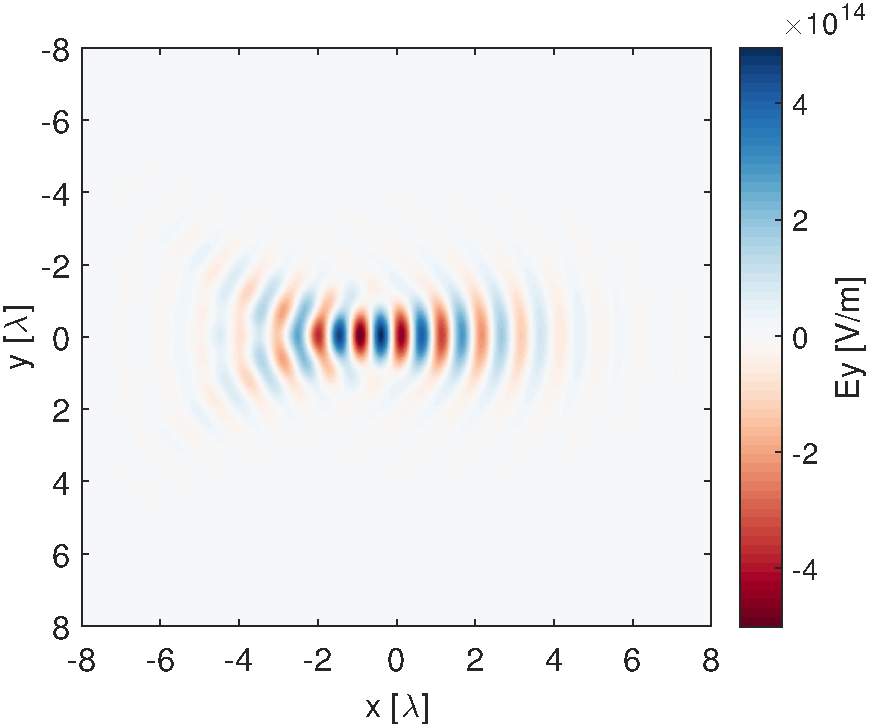
\includegraphics[width=0.44\linewidth]{./img/parax/Ey_focus.pdf}}}
	\hspace{2mm}
	\sidesubfloat[]{{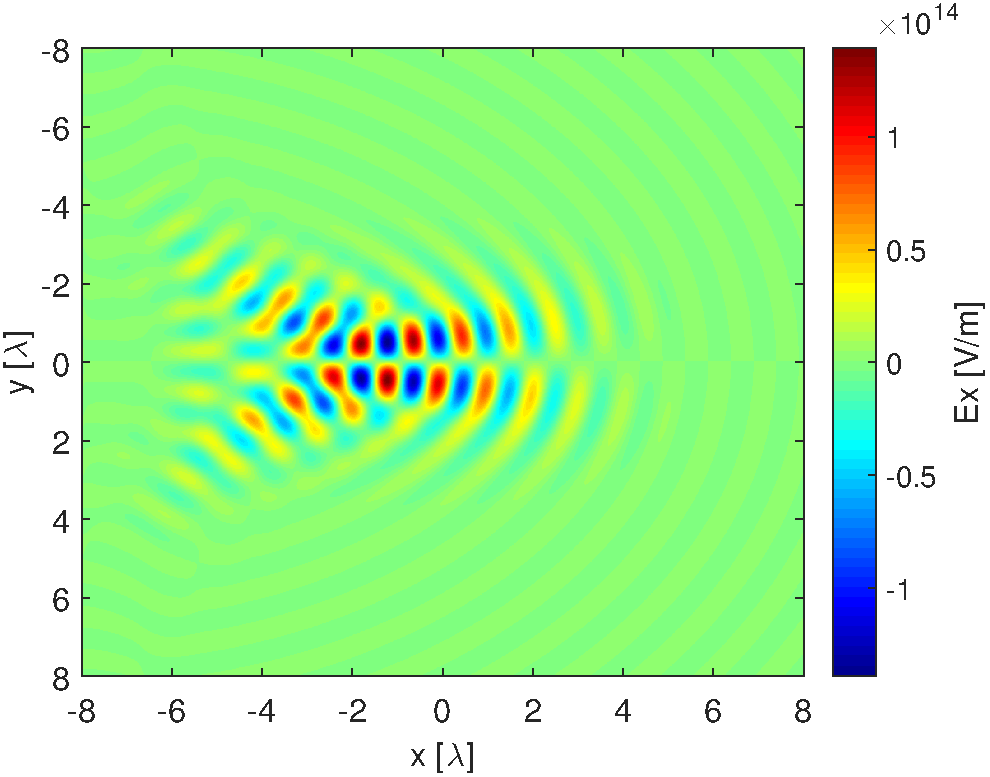
\includegraphics[width=0.44\linewidth]{./img/parax/Ex_focus.pdf}}}\\
	\sidesubfloat[]{{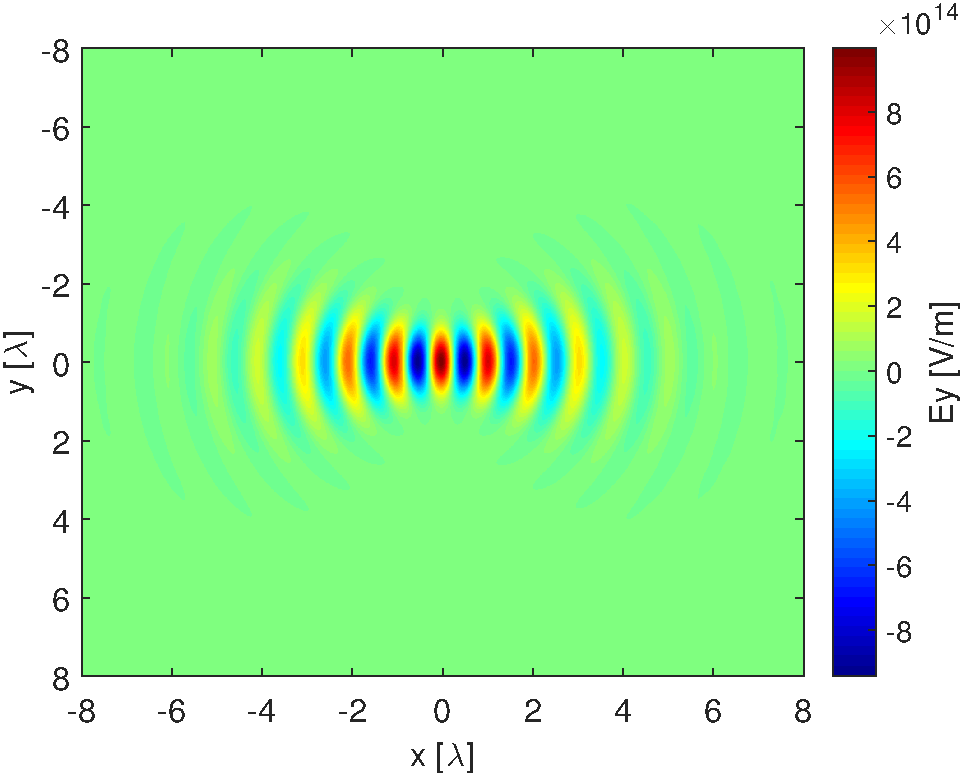
\includegraphics[width=0.44\linewidth]{./img/lbcs/Ey_focus.pdf}}}
	\hspace{2mm}
	\sidesubfloat[]{{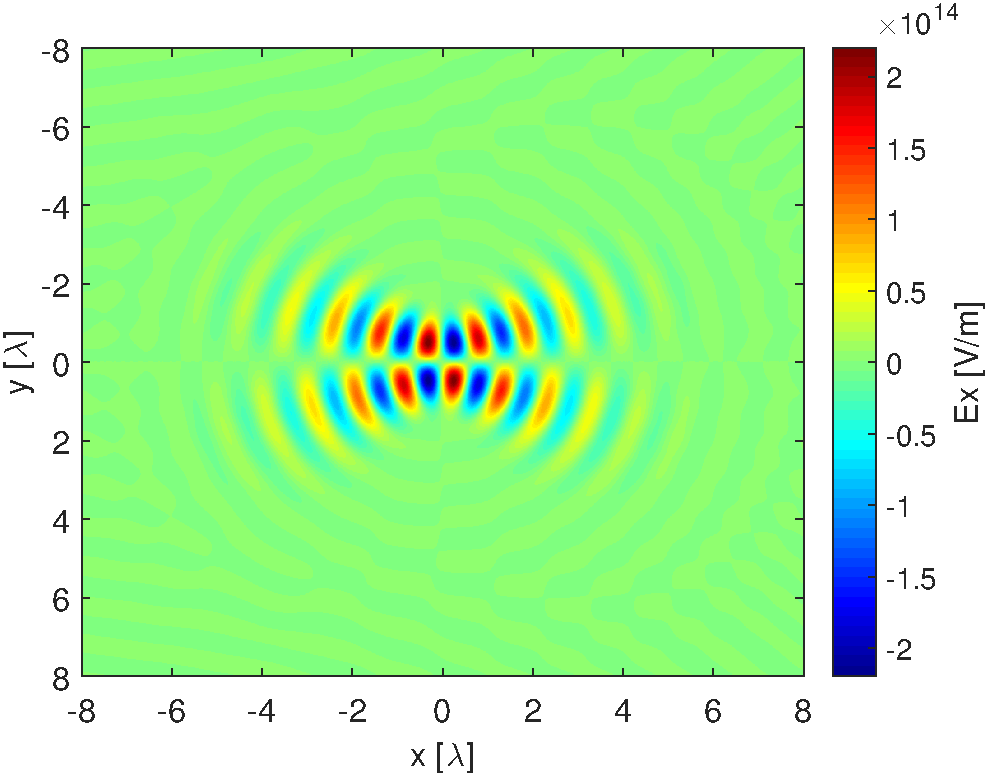
\includegraphics[width=0.44\linewidth]{./img/lbcs/Ex_focus.pdf}}}
	\caption{Transverse ($ E_{y} $) and longitudinal ($ E_{x} $) electric laser field components captured at the time step of their maximal intensity in the focal spot. The cases \textbf{(a)}, \textbf{(b)} correspond to the laser pulse propagating under the paraxial approximation, whilst \textbf{(c)}, \textbf{(d)} come from the simulation where the beam propagation has been resolved within the Maxwell consistent approach. In the case of paraxial approximation, both components reveal strong distortions and asymmetry, their focal spot is located about $ \mathrm{1 \mu m} $ closer to the left boundary than specified and the corresponding amplitude is significantly higher. The laser has been attached to the left hand side boundary.}
	\label{fig:1}
\end{figure}

\floatsetup[figure]{style=plain, subcapbesideposition=top}
\begin{figure}[h!]
	\centering
	\sidesubfloat[]{{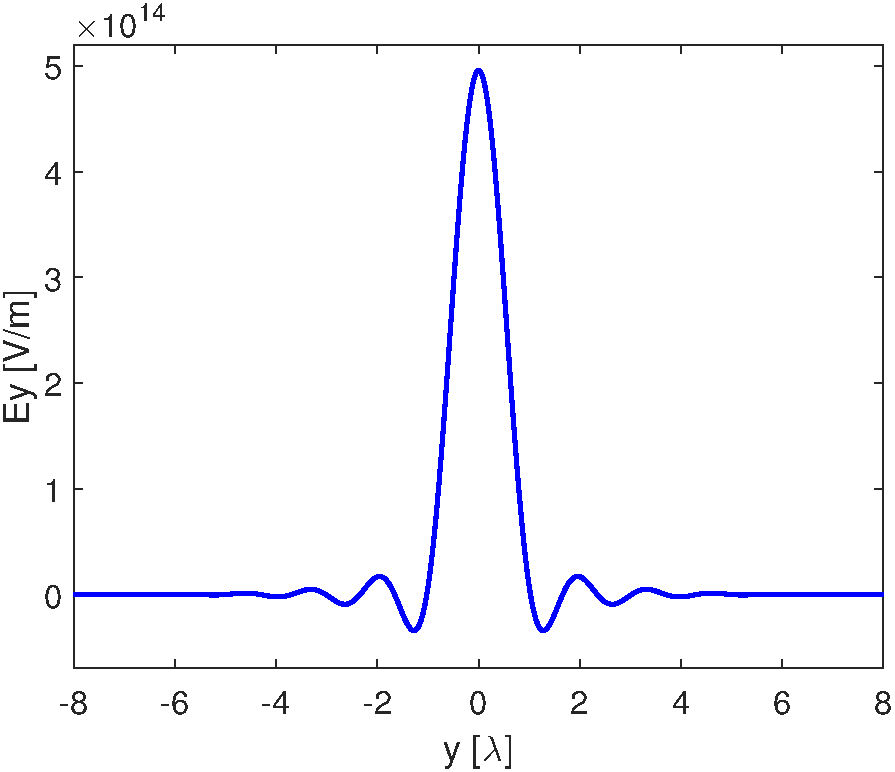
\includegraphics[width=0.4\linewidth]{./img/parax/Ey_focus_trans.pdf}}}
	\hspace{5mm}
	\sidesubfloat[]{{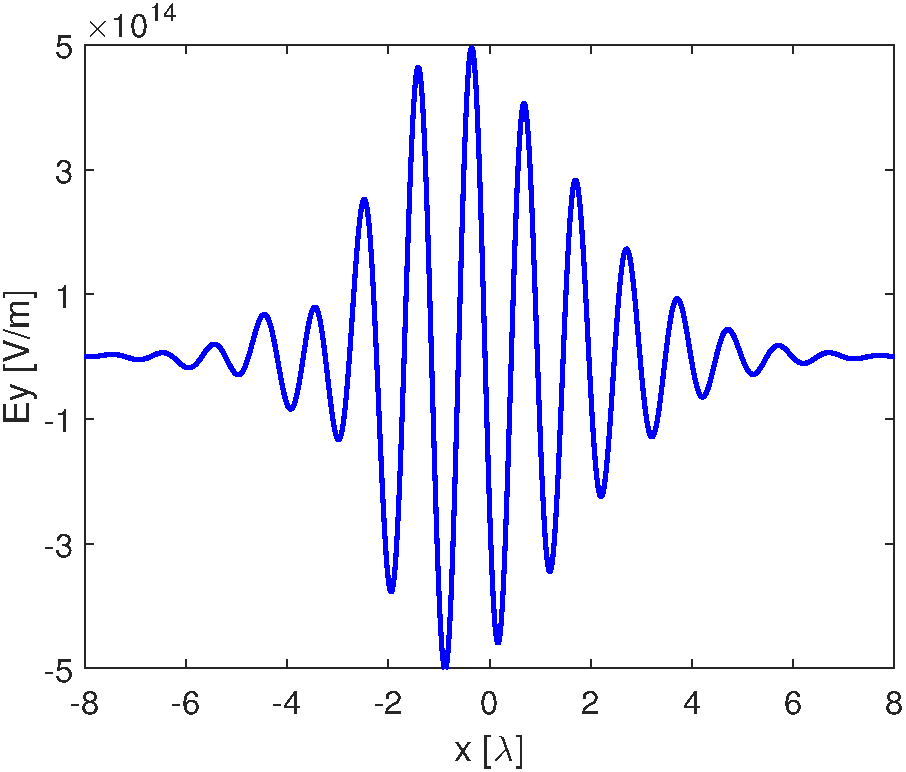
\includegraphics[width=0.4\linewidth]{./img/parax/Ey_focus_long.pdf}}}\\
	\sidesubfloat[]{{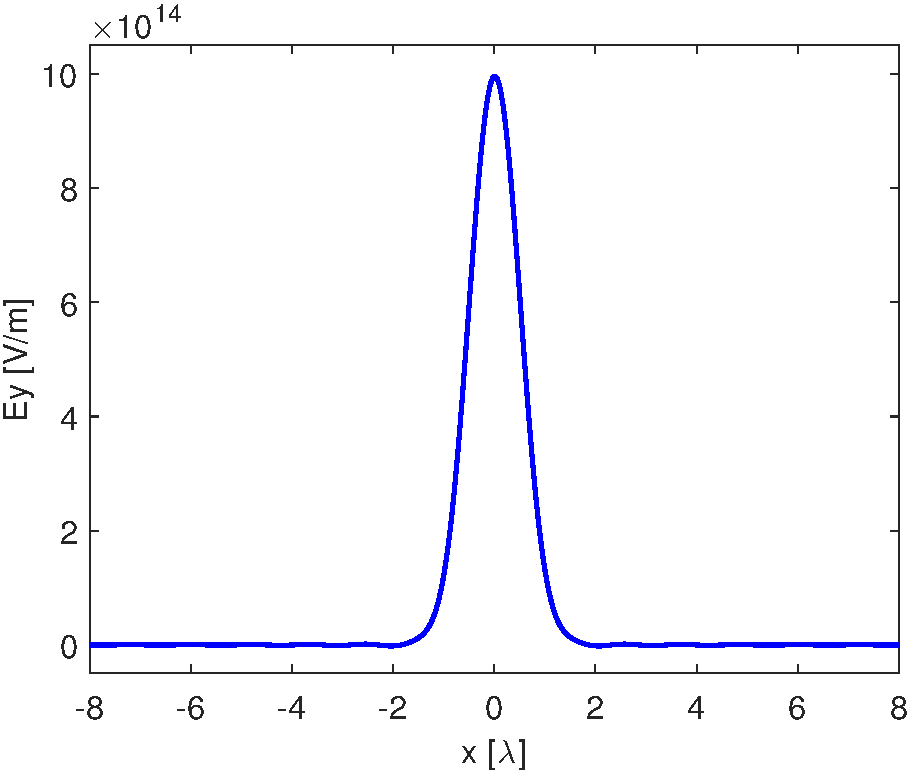
\includegraphics[width=0.4\linewidth]{./img/lbcs/Ey_focus_trans.pdf}}}
	\hspace{5mm}
	\sidesubfloat[]{{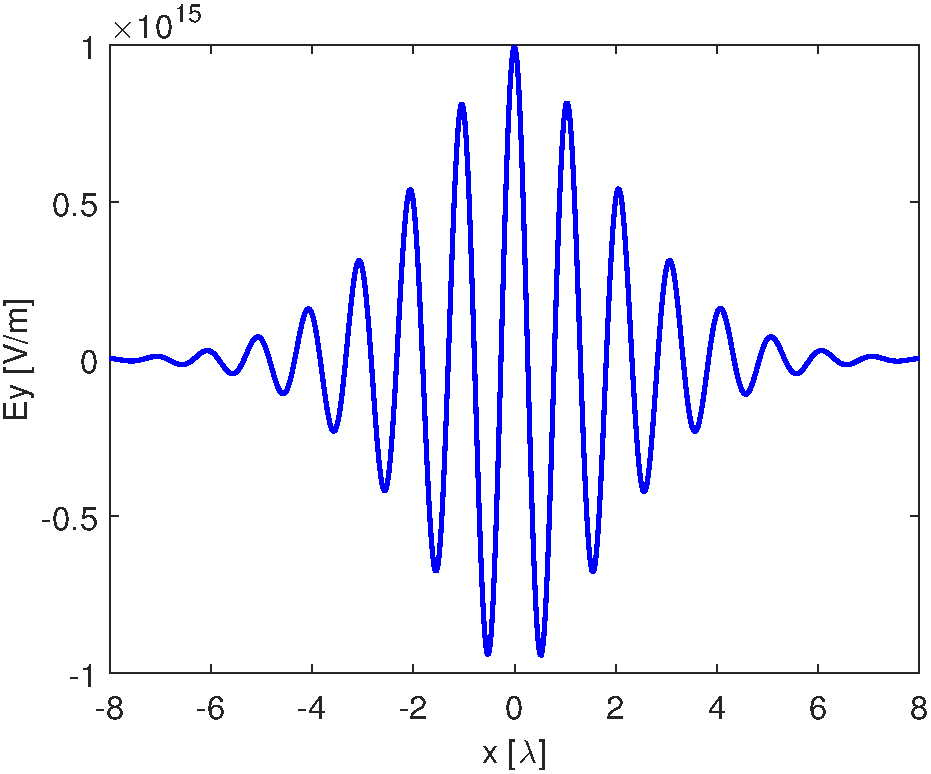
\includegraphics[width=0.4\linewidth]{./img/lbcs/Ey_focus_long.pdf}}}
	\caption{Transverse \textbf{(a)}, \textbf{(c)} and longitudinal \textbf{(b)}, \textbf{(d)} slices of the transverse electric laser field ($ E_{y} $) at the time step when it reaches maximal intensity in the focal spot. The cases \textbf{(a)}, \textbf{(b)} correspond to the laser pulse propagating under the paraxial approximation, whilst \textbf{(c)}, \textbf{(d)} come from the simulation where the beam propagation has been resolved within the Maxwell consistent approach. In the case of paraxial approximation, one can clearly see strong side-wings in the spatial beam profile \textbf{(a)} as well as the asymmetry of the field in the longitudinal line-out \textbf{(b)}.}
	\label{fig:2}
\end{figure}

\floatsetup[figure]{style=plain, subcapbesideposition=top}
\begin{figure}[h!]
	\centering
	\sidesubfloat[]{{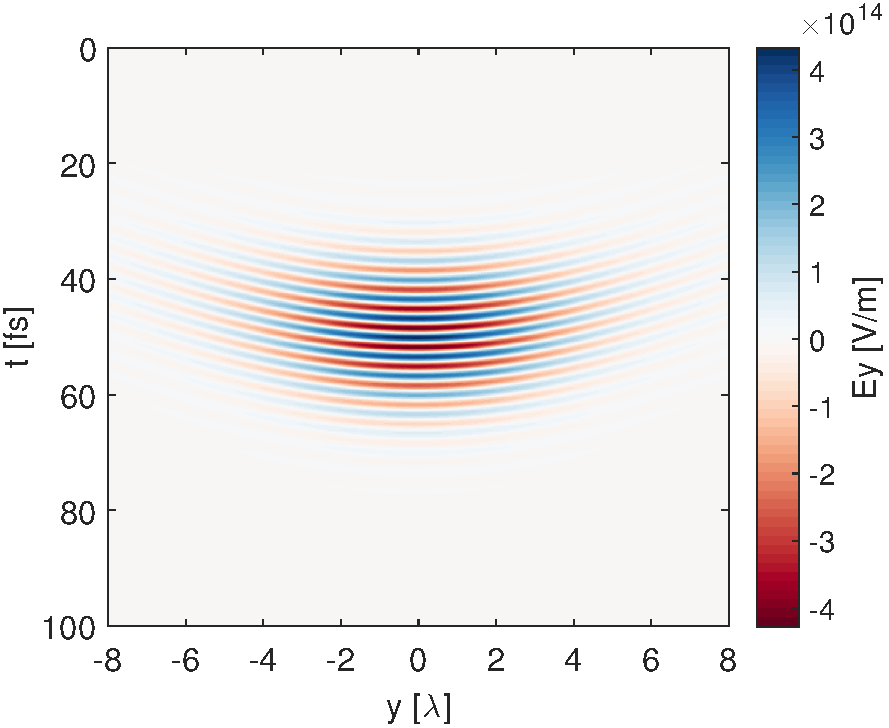
\includegraphics[width=0.44\linewidth]{./img/lbcs/Ey_boundary_time.pdf}}}
	\hspace{2mm}
	\sidesubfloat[]{{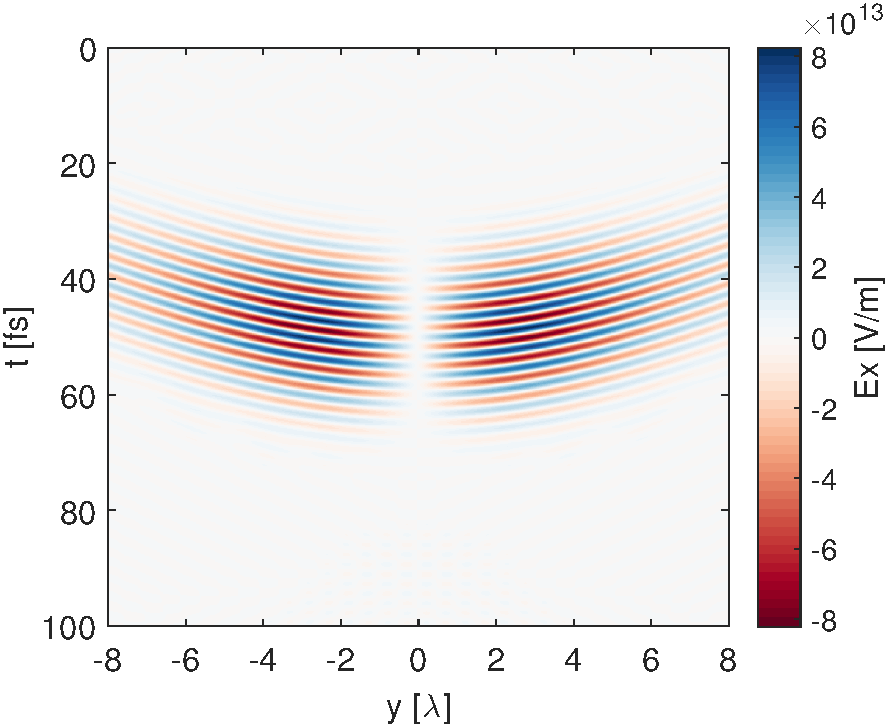
\includegraphics[width=0.44\linewidth]{./img/lbcs/Ex_boundary_time.pdf}}}
	\caption{The time evolution of transverse ($ E_{y} $) \textbf{(a)} and longitudinal ($ E_{x} $) \textbf{(b)} electric laser field components at the boundary that the laser is attached to. Both components has been calculated according to the Maxwell consistent approach.}
	\label{fig:3}
\end{figure}

\floatsetup[figure]{style=plain, subcapbesideposition=top}
\begin{figure}[h!]
	\centering
	\sidesubfloat[]{{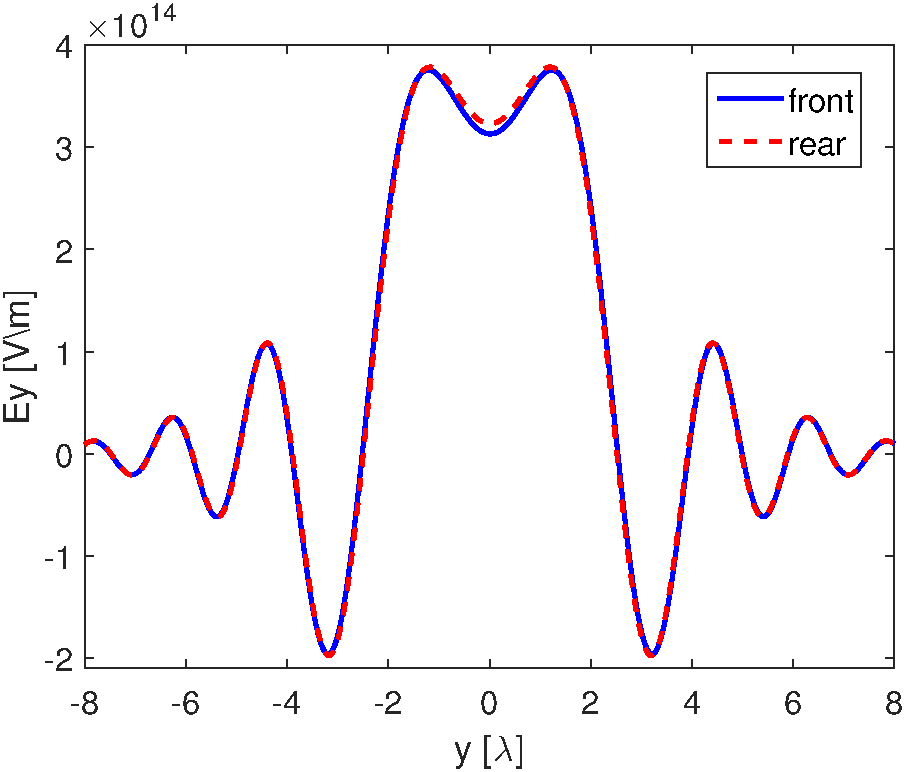
\includegraphics[width=0.44\linewidth]{./img/lbcs/Ey_boundary_trans.pdf}}}
	\hspace{1mm}
	\sidesubfloat[]{{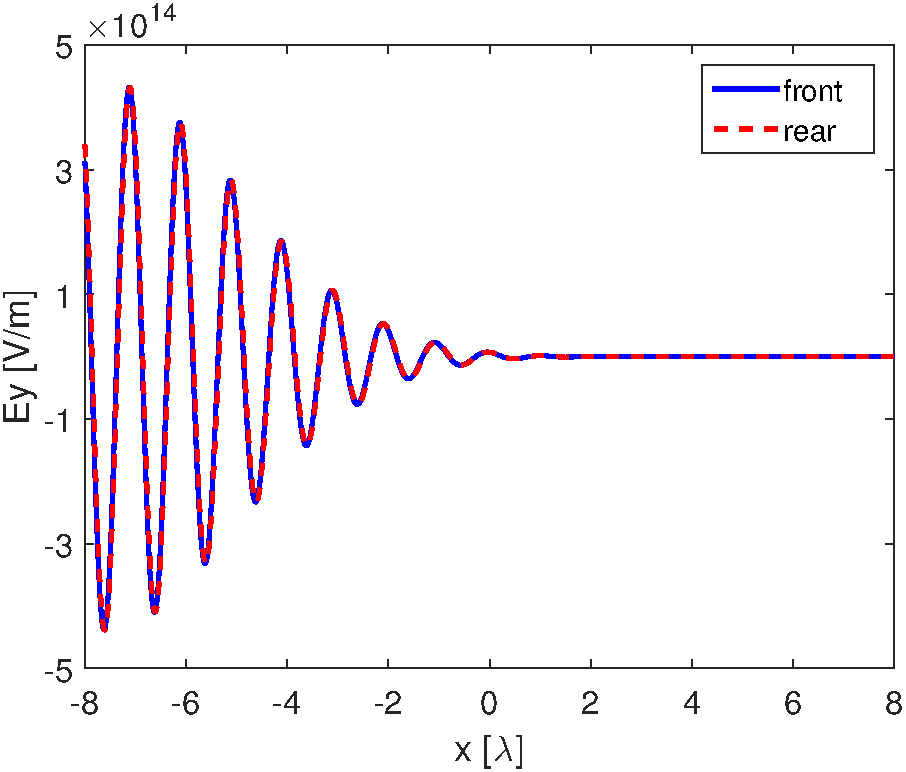
\includegraphics[width=0.44\linewidth]{./img/lbcs/Ey_boundary_long.pdf}}}
	\caption{Transverse \textbf{(a)} and longitudinal \textbf{(b)} slice of the transverse electric laser field ($ E_{y} $) when it reaches its maximal intensity at the front (blue) and rear (red) boundary. The results come from the simulation where the Maxwell consistent approach for laser propagation has been used. For better comparison, the field at the rear boundary in \textbf{(b)} has been horizontally flipped. The exact match between the field shapes at a different time steps of simulation proves the correctness of the laser beam propagation.}
	\label{fig:4}
\end{figure}

\floatsetup[figure]{style=plain, subcapbesideposition=top}
\begin{figure}[h!]
	\centering
	\sidesubfloat[]{{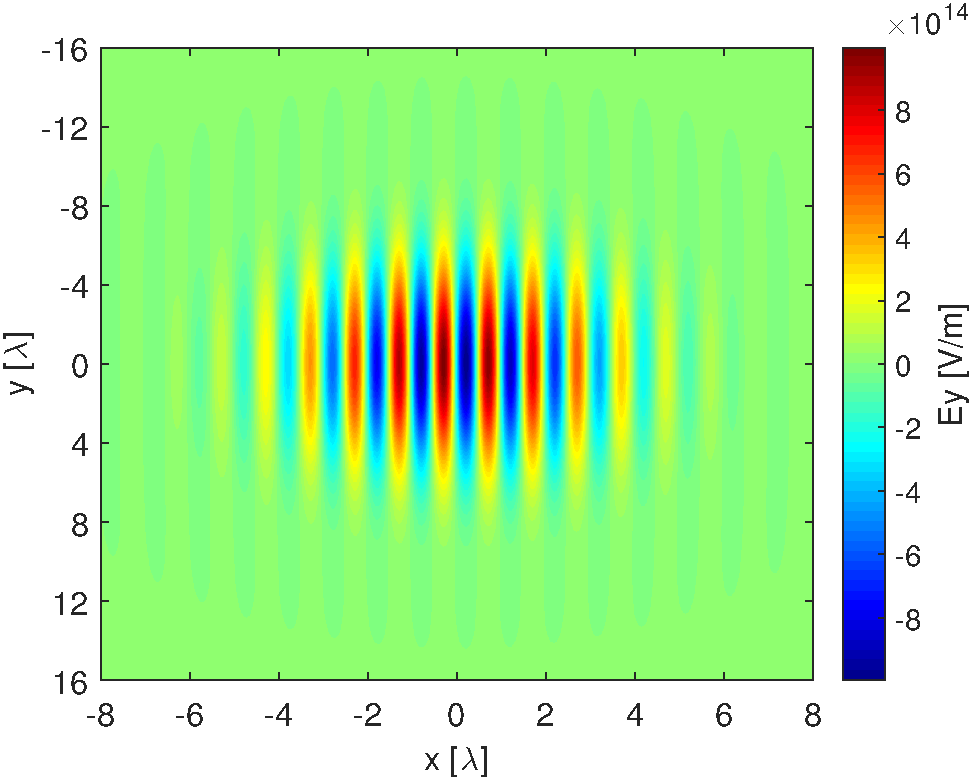
\includegraphics[width=0.45\linewidth]{./img/parax/Ey_focus_5mic.pdf}}}
	\hspace{2mm}
	\sidesubfloat[]{{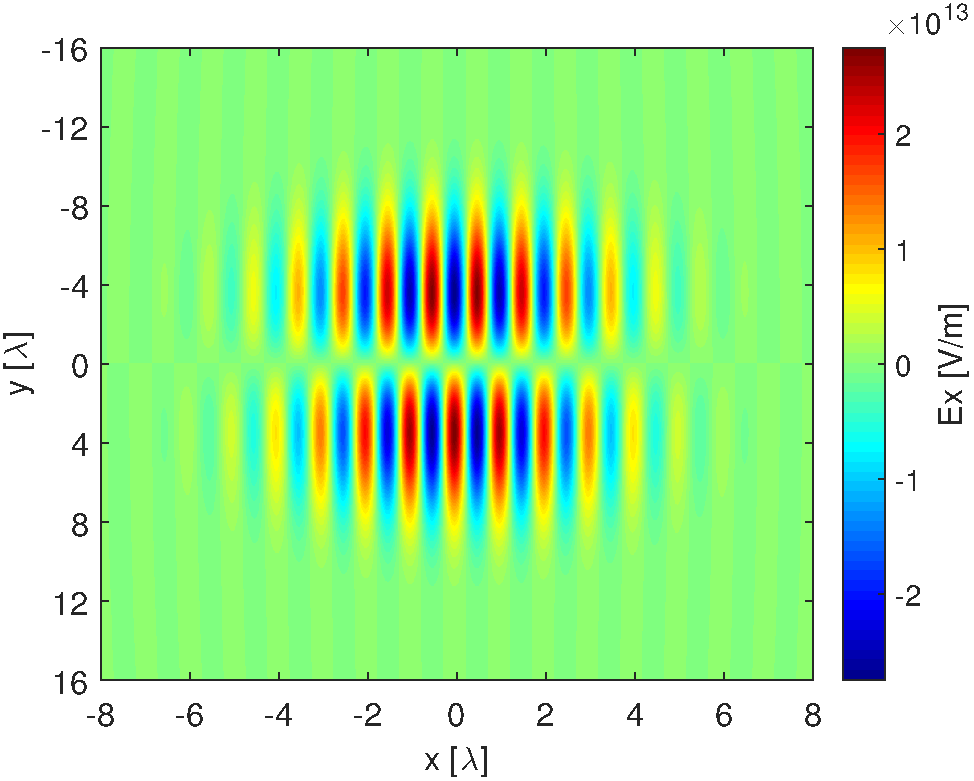
\includegraphics[width=0.44\linewidth]{./img/parax/Ex_focus_5mic.pdf}}}\\
	\sidesubfloat[]{{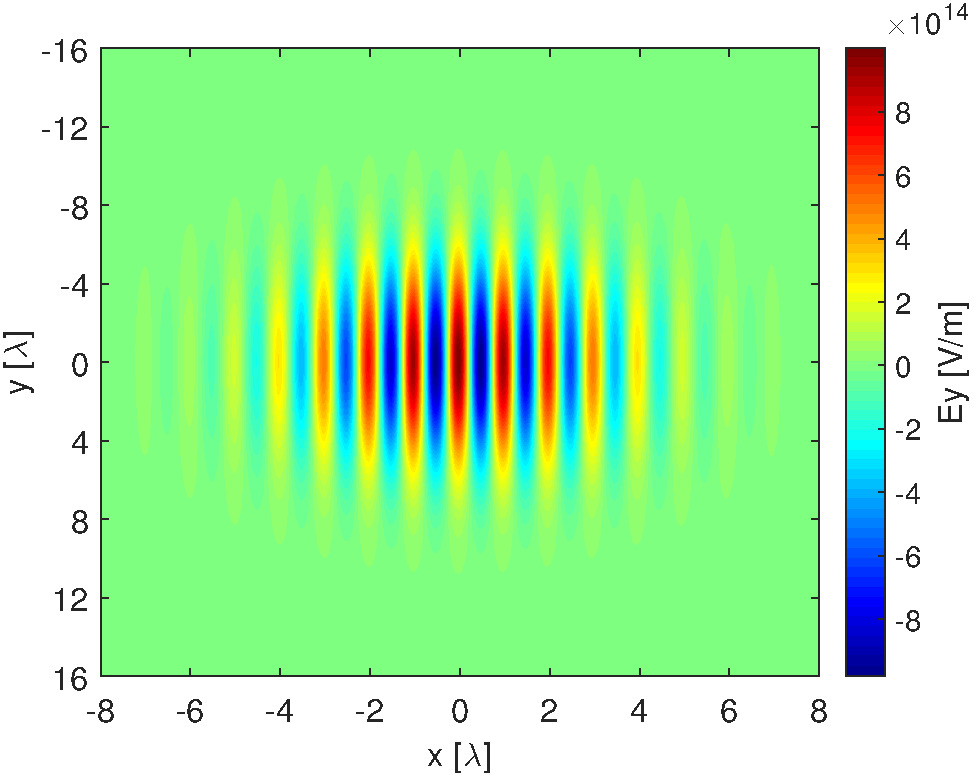
\includegraphics[width=0.44\linewidth]{./img/lbcs/Ey_focus_5mic.pdf}}}
	\hspace{2mm}
	\sidesubfloat[]{{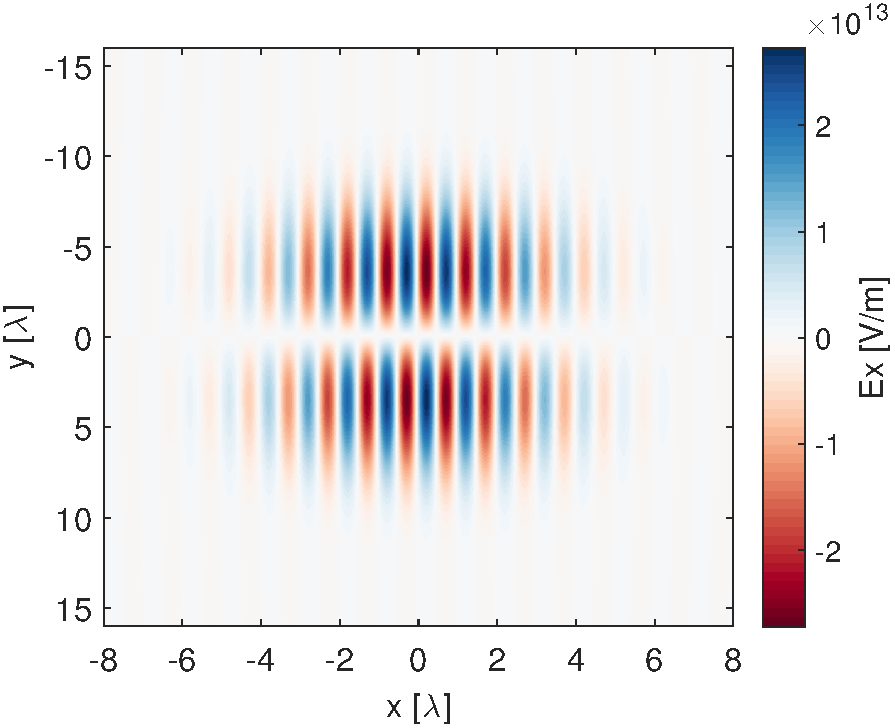
\includegraphics[width=0.43\linewidth]{./img/lbcs/Ex_focus_5mic.pdf}}}
	\caption{Transverse ($ E_{y} $) and longitudinal ($ E_{x} $) electric laser field components captured at the time step of their maximal intensity in the focal spot. The cases \textbf{(a)}, \textbf{(b)} correspond to the laser pulse propagating under the paraxial approximation, whilst \textbf{(c)}, \textbf{(d)} come from the simulation where the beam propagation has been resolved within the Maxwell consistent approach. The size of the focus has been chosen to be one order of the magnitude larger than the center laser wavelength. One can clearly see, that there is no significant difference between the shapes of the electric field components.}
	\label{fig:5}
\end{figure}

\floatsetup[figure]{style=plain, subcapbesideposition=top}
\begin{figure}[h!]
	\centering
	\sidesubfloat[]{{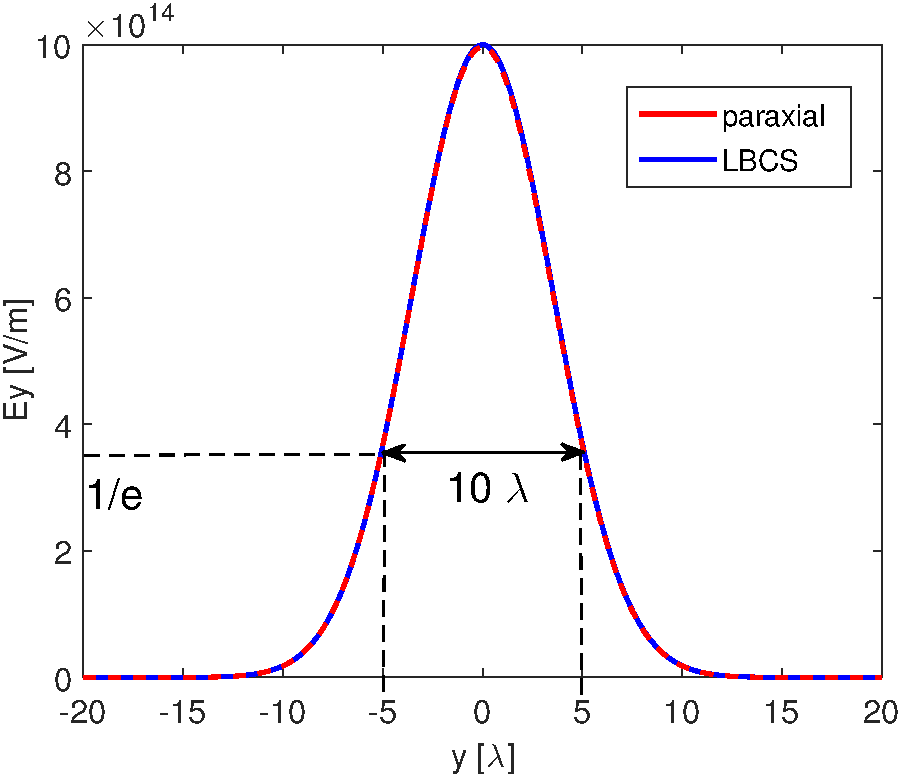
\includegraphics[width=0.44\linewidth]{./img/parax/Ey_focus_trans_comparison.pdf}}}
	\hspace{1mm}
	\sidesubfloat[]{{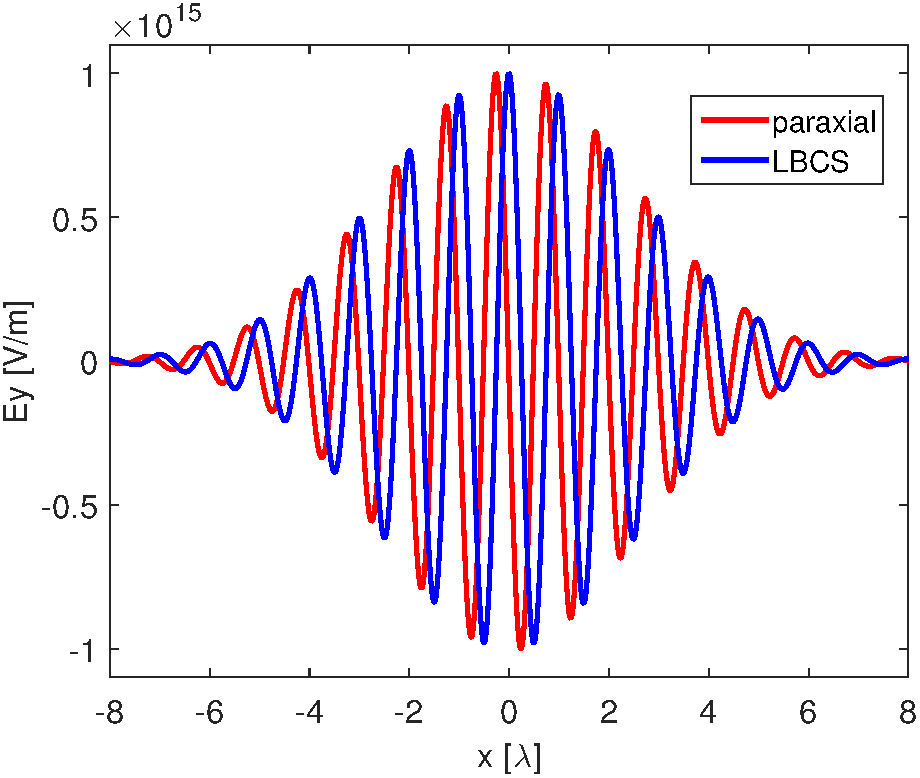
\includegraphics[width=0.45\linewidth]{./img/parax/Ey_focus_long_comparison.pdf}}}
	\caption{Transverse \textbf{(a)} and longitudinal \textbf{(b)} slices of the transverse electric laser field ($ E_{y} $) at the time step when it reaches maximal intensity in the focal spot. Red lines correspond to the laser pulse propagating under the paraxial approximation, whilst blue lines come from the simulation where the beam propagation has been resolved within the Maxwell consistent approach. The size of the focus has been chosen to be one order of magnitude larger than the center laser wavelength. In the case of paraxial approximation, the focus is slightly shifted closer to the left boundary \textbf{(b)}, otherwise the size of the focus as well as the amplitude is correct for both cases \textbf{(a)}.}
	\label{fig:6}
\end{figure}
